\section{Experimental setup}
 

In order to determine the tire characteristics of the scaled vehicle, a good testbed is necessary. In this section the experimental setup used to gather the data needed for determining the tire characteristic is discussed.\\
The experimental setup consists of a modified scaled RC car with an on board IMU, and a tachometer on each wheel. Moreover, a motion capture system or MoCap was used to provide millimeter precision locating. A note should be made here that the testbed was recycled from earlier research into the same subject made by [reference to last group's paper]. As stated in their paper there were a lot of software related problems with the car. Therefore the limited time we had for this research, was mostly used for programming the test setup and creating a working system. We therefore choose to ignore any physical design faults, at least in the beginning, to fix these problems first. This made our results susceptible to these faults in the end. Later work might improve on this. 

Usually a MoCap system can't be regarded as an \textquotesingle on-board sensor\textquotesingle ,seeing as it requires an external area with set up with camera's. However in our case it was used as a replacement for a gps sensor. A gps sensor would be less desirable in our situation as the accuracy doesn't scale down with the car. Moreover a MoCap system enables us to do testing inside. Something which is troubling at best when tried with a GPS system. Moreover, most of the MoCap system was delivered as is. Which meant all of the data would be presented in ROS. And the sampling rate of the mocap would be set in stone at 120HZ.

The scaled RC car is a Losi TEN Rally-X. It is a 1:10 scale car with 4WD.  
Each wheel was fitted with it\textquotesingle s own hall effect sensor which generates a pulse every time one of the magnets inside the rim passes it. Many of the first tests were done using only 2 magnets giving only 1 pulse per \(pi\) radial turned. However after most of the testing was done we figured out a rim with 24 magnets would be much more suited. To fit both the 2 magnets and the 24 magnet versions to the car a set of custom 3d printed rims were created. Using the 24 magnet version a pulse every \(pi/12\) radial was generated giving a higher resolution. Finally, the car\textquotesingle s suspension is replaced with stiff turnbuckle rods to eliminate the degrees of freedom of roll and pitch, to meet the assumptions of the Bicycle model.

\begin{figure}
  \centering
    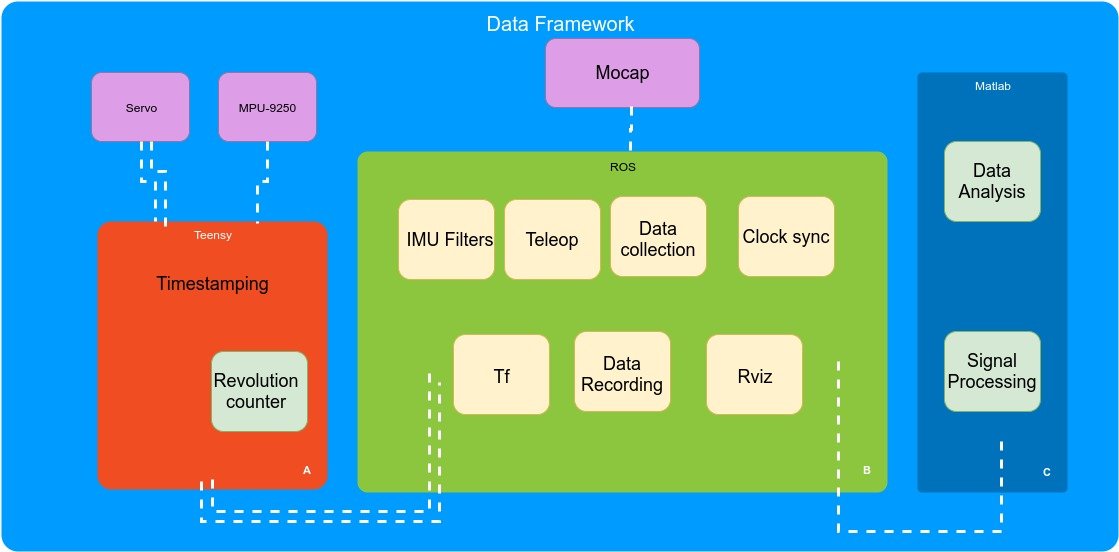
\includegraphics[scale=0.22]{figure/DataFramework.jpg}
  \caption{Data acquisition framework}
  \label{fig:DonutFramework} 
\end{figure}

Data acquisition was done using a ROS (Robot Operating System) based system. The sensors were read using a Teensy 3.6 protyping board running a costum ROSserial node, connected to a Raspberry pi 3b running ROS. The MoCap connected to the system utilizig the labs Wi-Fi network. Further communication was done using a self written ROS package. After data collection further processing was done using Matlab.Figure
\ref{fig:DonutFramework} further eleborates the Data acquisition framework.

ROS was chosen as basis for the system for 3 reasons. First, there was already a lot of experience in the research team using ROS which made it an easy choice to use to fix a lot of the problems with the testbed. Second the MoCap generated it's data already in ROS. Which meant combining everything in ROS would be a simplification. Last ROS offers really easy Data recording options called ROSbags. These can be easily imported in to MATLAB to do further analysis.

Seeing as the MoCap already delivered her data at a sampling rate of 120hz. It was easy to pick this as the target sampling rate for the whole system. Seeing as our speeds reach somewhere in between 0-20[m/s] this would mean a maximum of 0.167[m] traveled per sample. This felt accurate enough for our purpose.

The experiments that we conducted can be classified into three groups. The first set of experiments are the ones on the straight (longitudinal motion). During these we accelerated and braked while driving straight ahead. The second set are the steady state cornering experiments (lateral motion). Steady state cornering means cornering at a constant longitudinal velocity and constant steering angle. The first group of experiments focuses on longitudinal forces and slip ratios, while the second group focuses on lateral forces and slip angles. The tests were separated in order to distinguish longitudinal and lateral motion (Recommendation Barys Shyrokau). Finally, the third set of experiments are of combined motion. These tests take both lateral and longitudinal motion into account. 
	Variables of the tests are acceleration/deceleration for longitudinal motion, longitudinal velocity and steering angle for lateral motion, and these three combined for  combined motion. The variables were slightly increased each experiment in order to determine the \textquotesingle borderline\textquotesingle  between linear and nonlinear behaviour is.
	
The experimental data is collected in rosbags and processed afterwards. This makes it possible to filter the noise from the IMU with a Zero-Phase Low Pass Butterworth Filter. This is a non-causal filter with a phase slope of zero. This eliminates any delay, commonly caused by causal filters. The Low Pass filter is of the 20th order, in order to approach an ideal \textquotesingle Brick wall Response\textquotesingle .
	\begin{figure}
	\centering
	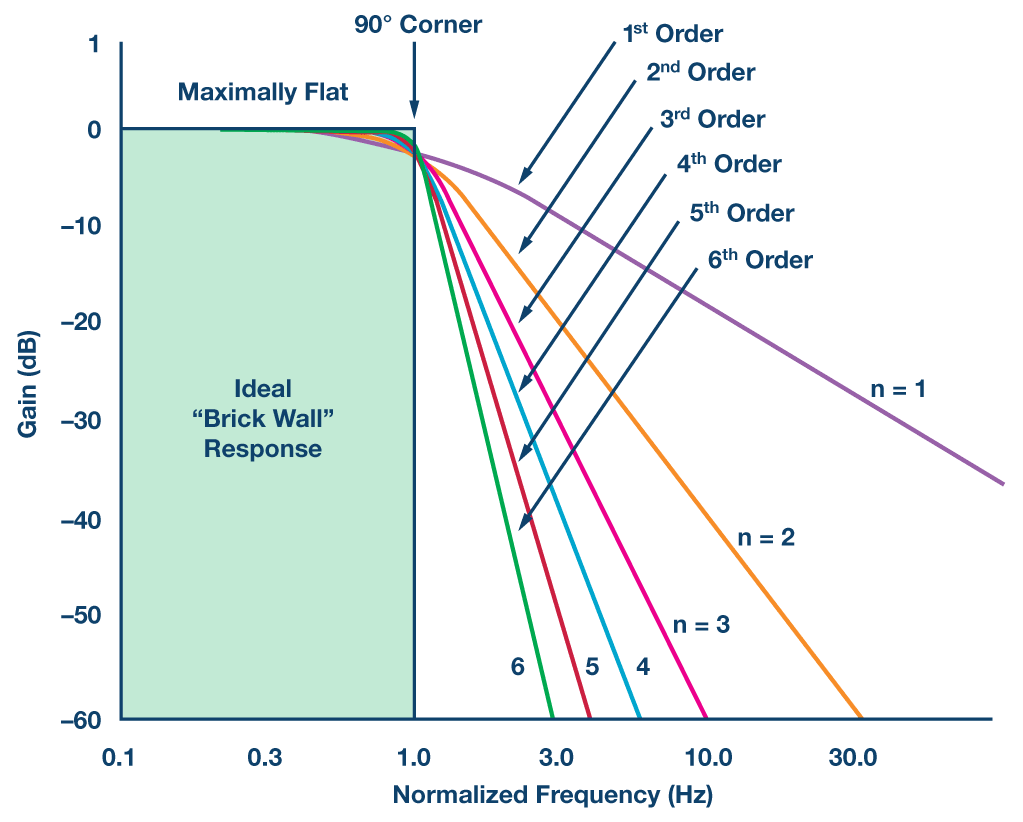
\includegraphics[scale=0.17]{figure/brickwall.png}
	\caption{Brick wall response}
	%\captionsource{Caption}{(http://www.electronics-tutorials.ws/filter/filter_8.html)}
	\label{fig:brickwall}
	\end{figure}


 
\subsection{Longitudinal slip}
Differentiating the Mocap Data creates a lot of noise. Integrating the IMU data results in a much more stable velocity signal. This signal combined with the data from the Hall Effect Sensors is used to calculate the Longitudinal slip ratio using the following formulas:
\begin{figure}
	\centering
	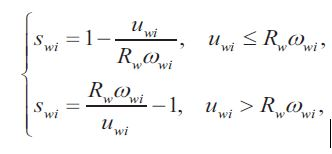
\includegraphics[scale=0.4]{figure/Longitudonalslip}
	\caption{Longitudinal slip}
	\label{fig:brickwall}
	\end{figure}

\subsection{Forces}
The forces, acting along the y-axis of the body fixed frame of the car, are calculated using the equations of motion. As mentioned earlier there are three types of experiments that were conducted. This makes it easier to obtain these forces.

\begin{figure}
	\centering
	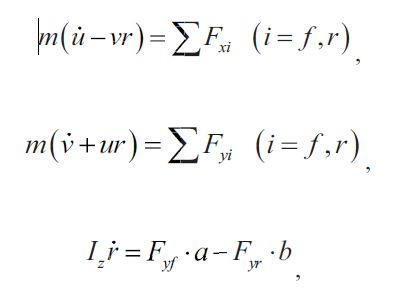
\includegraphics[scale=0.4]{figure/Equationsofmotion}
	\caption{equations of motion}
	\label{fig:brickwall}
	\end{figure}

Where the forces on the wheels are obtained by formula \ref{eq:magicformula}

\subsection{Curve Fitting}
After obtaining the forces, slip ratio and slip angles, from multiple bags, the data is curve fitted in order to obtain the 4 parameters from the magic formula.
 

